\section{Statistiques descriptives}

\subsection{Variables démographiques}

\subsubsection*{Tableaux de fréquences}
Les tableaux de fréquences ci-après (\autoref{tab:freq1} et \autoref{tab:freq2}) présentent la distribution de la variable suicidaire selon le sexe (femme vs. homme) et selon la variable hétérosexuel (non vs. oui). Chaque cellule indique le nombre d’individus appartenant à la catégorie en ligne et en colonne correspondante. Ces comptes permettent d’apprécier la répartition conjointe de deux caractéristiques (p.~ex.~sexe et suicidaire) et d’identifier d’éventuelles différences de fréquence entre les groupes.

\begin{table}[H]
	\centering
	\caption{Distribution de la variable suicidaire selon le sexe.}
	\label{tab:freq1}
	\begin{tabular}{|rr|cc|}
		\toprule
		   & & \multicolumn{2}{c|}{\textbf{Suicidaire}} \\
		  & & Non & Oui \\
		\midrule
	\textbf{Sexe}	& Femme & 4 & 4 \\
					& Homme & 4 & 4 \\
		\bottomrule
	\end{tabular}
\end{table}

\begin{table}[H]
	\centering
	\caption{Distribution de la variable suicidaire selon la hétérosexualité.}
	\label{tab:freq2}
	\begin{tabular}{|rr|cc|}
		\toprule
		& & \multicolumn{2}{c|}{\textbf{Suicidaire}} \\
		& & Non & Oui\\
		\midrule
\textbf{Hétérosexualité} & Non & 3 & 2 \\
		& Oui & 5 & 6 \\
		\bottomrule
	\end{tabular}
\end{table}


\subsubsection*{Moyennes de la variable suicidaire}
En complément de ces tableaux de fréquences, la proportion d’individus suicidaires a été calculé dans différents sous-groupes de la population étudiée : hommes, femmes, hétérosexuels et non-hétérosexuels. Les résultats, présentés dans le tableau~\ref{tab:moyennes-suicidal}, indiquent que :

\begin{itemize}
	\item Le taux de suicidaires est de 50\% tant chez les hommes que chez les femmes.
	\item Les hétérosexuels présentent un taux moyen légèrement plus élevé (environ 55\%) que les non-hétérosexuels (environ 40\%).
\end{itemize}

\begin{table}[H]
	\centering
	\caption{Proportion moyenne de la variable suicidaire selon le sexe et l’hétérosexualité.}
	\label{tab:moyennes-suicidal}
	\begin{tabular}{lc}
		\toprule
		\textbf{Sous-groupe} & \textbf{Moyenne} \\
		\midrule
		Hommes             & 0.50 \\
		Femmes             & 0.50 \\
		\hline
		Hétérosexuels      & 0.55 \\
		Non-hétérosexuels  & 0.40 \\
		\bottomrule
	\end{tabular}
\end{table}


\subsection{Variables émotionnelles}

Afin d’évaluer les différences d’intensité émotionnelle entre individus \og non suicidaires \fg{} et \og suicidaires \fg, dix variables ont été analysées : \emph{colère, anticipation, dégoût, peur, joie, tristesse, surprise, confiance, négatif et positif}. Deux approches ont été mises en œuvre : l’examen direct des valeurs observées (données originales) et l’estimation des moyennes via rééchantillonnage bootstrap.

\subsubsection{Approche avec données originales.}
Dans un premier temps, chaque émotion a été représentée sous forme de diagramme en boîtes (boxplot) pour les groupes \og non suicidaires \fg{} et \og suicidaires \fg. Cette visualisation permet de comparer la médiane, l’étendue interquartile et la présence éventuelle de valeurs atypiques pour chacune des dix émotions, comme le montre la Figure~\ref{fig:boxplot-emotions-suicidal-raw}.

\begin{figure}[H]
	\centering
	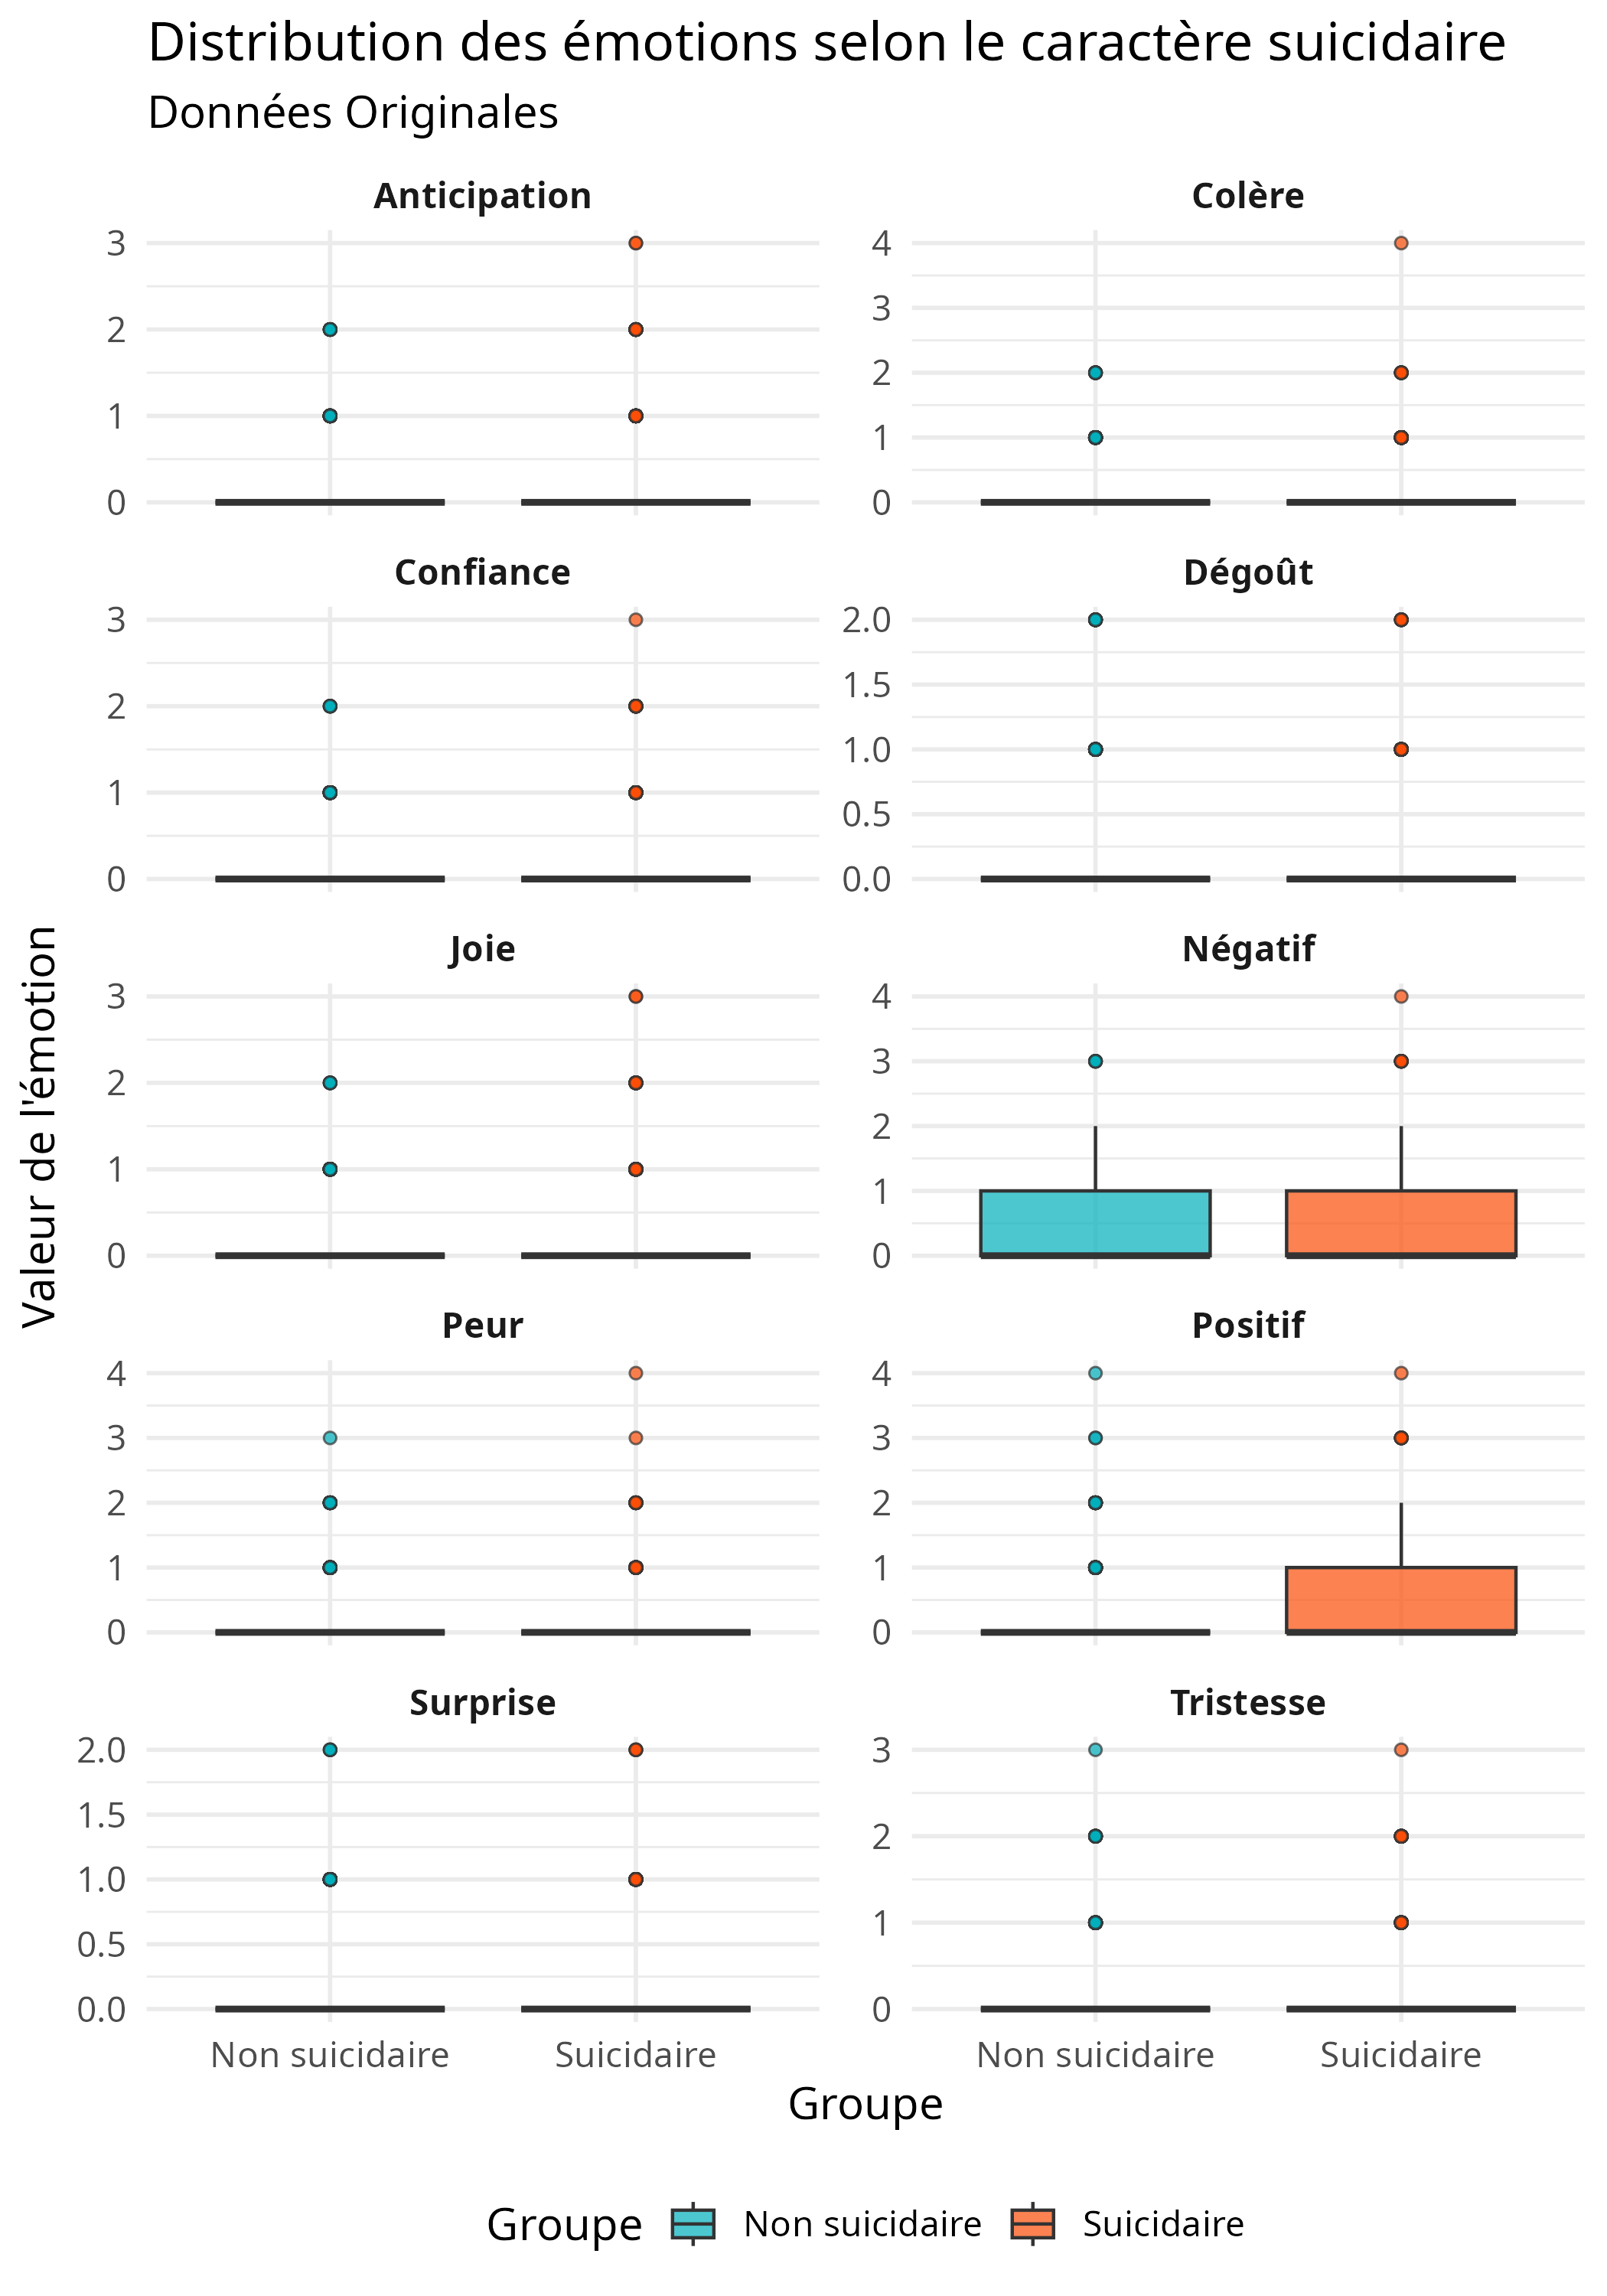
\includegraphics[width=0.8\textwidth]{images/boxplot-emotions-suicidal-raw.png}
	\caption{Distribution des émotions selon le caractère suicidaire (\emph{données originales}).}
	\label{fig:boxplot-emotions-suicidal-raw}
\end{figure}


\subsubsection{Approche par rééchantillonnage Bootstrap.}
Pour compléter cette analyse et apprécier la robustesse des estimations, un rééchantillonnage bootstrap a été réalisé à 10\,000 reprises. À chaque itération, un échantillon de même taille que l’échantillon initial est constitué \og avec remise \fg{}. Les moyennes des émotions sont alors recalculées séparément dans les deux groupes. Les distributions de ces moyennes (pour chaque émotion) sont illustrées par des diagrammes en boîtes dans la Figure~\ref{fig:boxplot-emotions-suicidal-bootstrap}.

\begin{figure}[H]
	\centering
	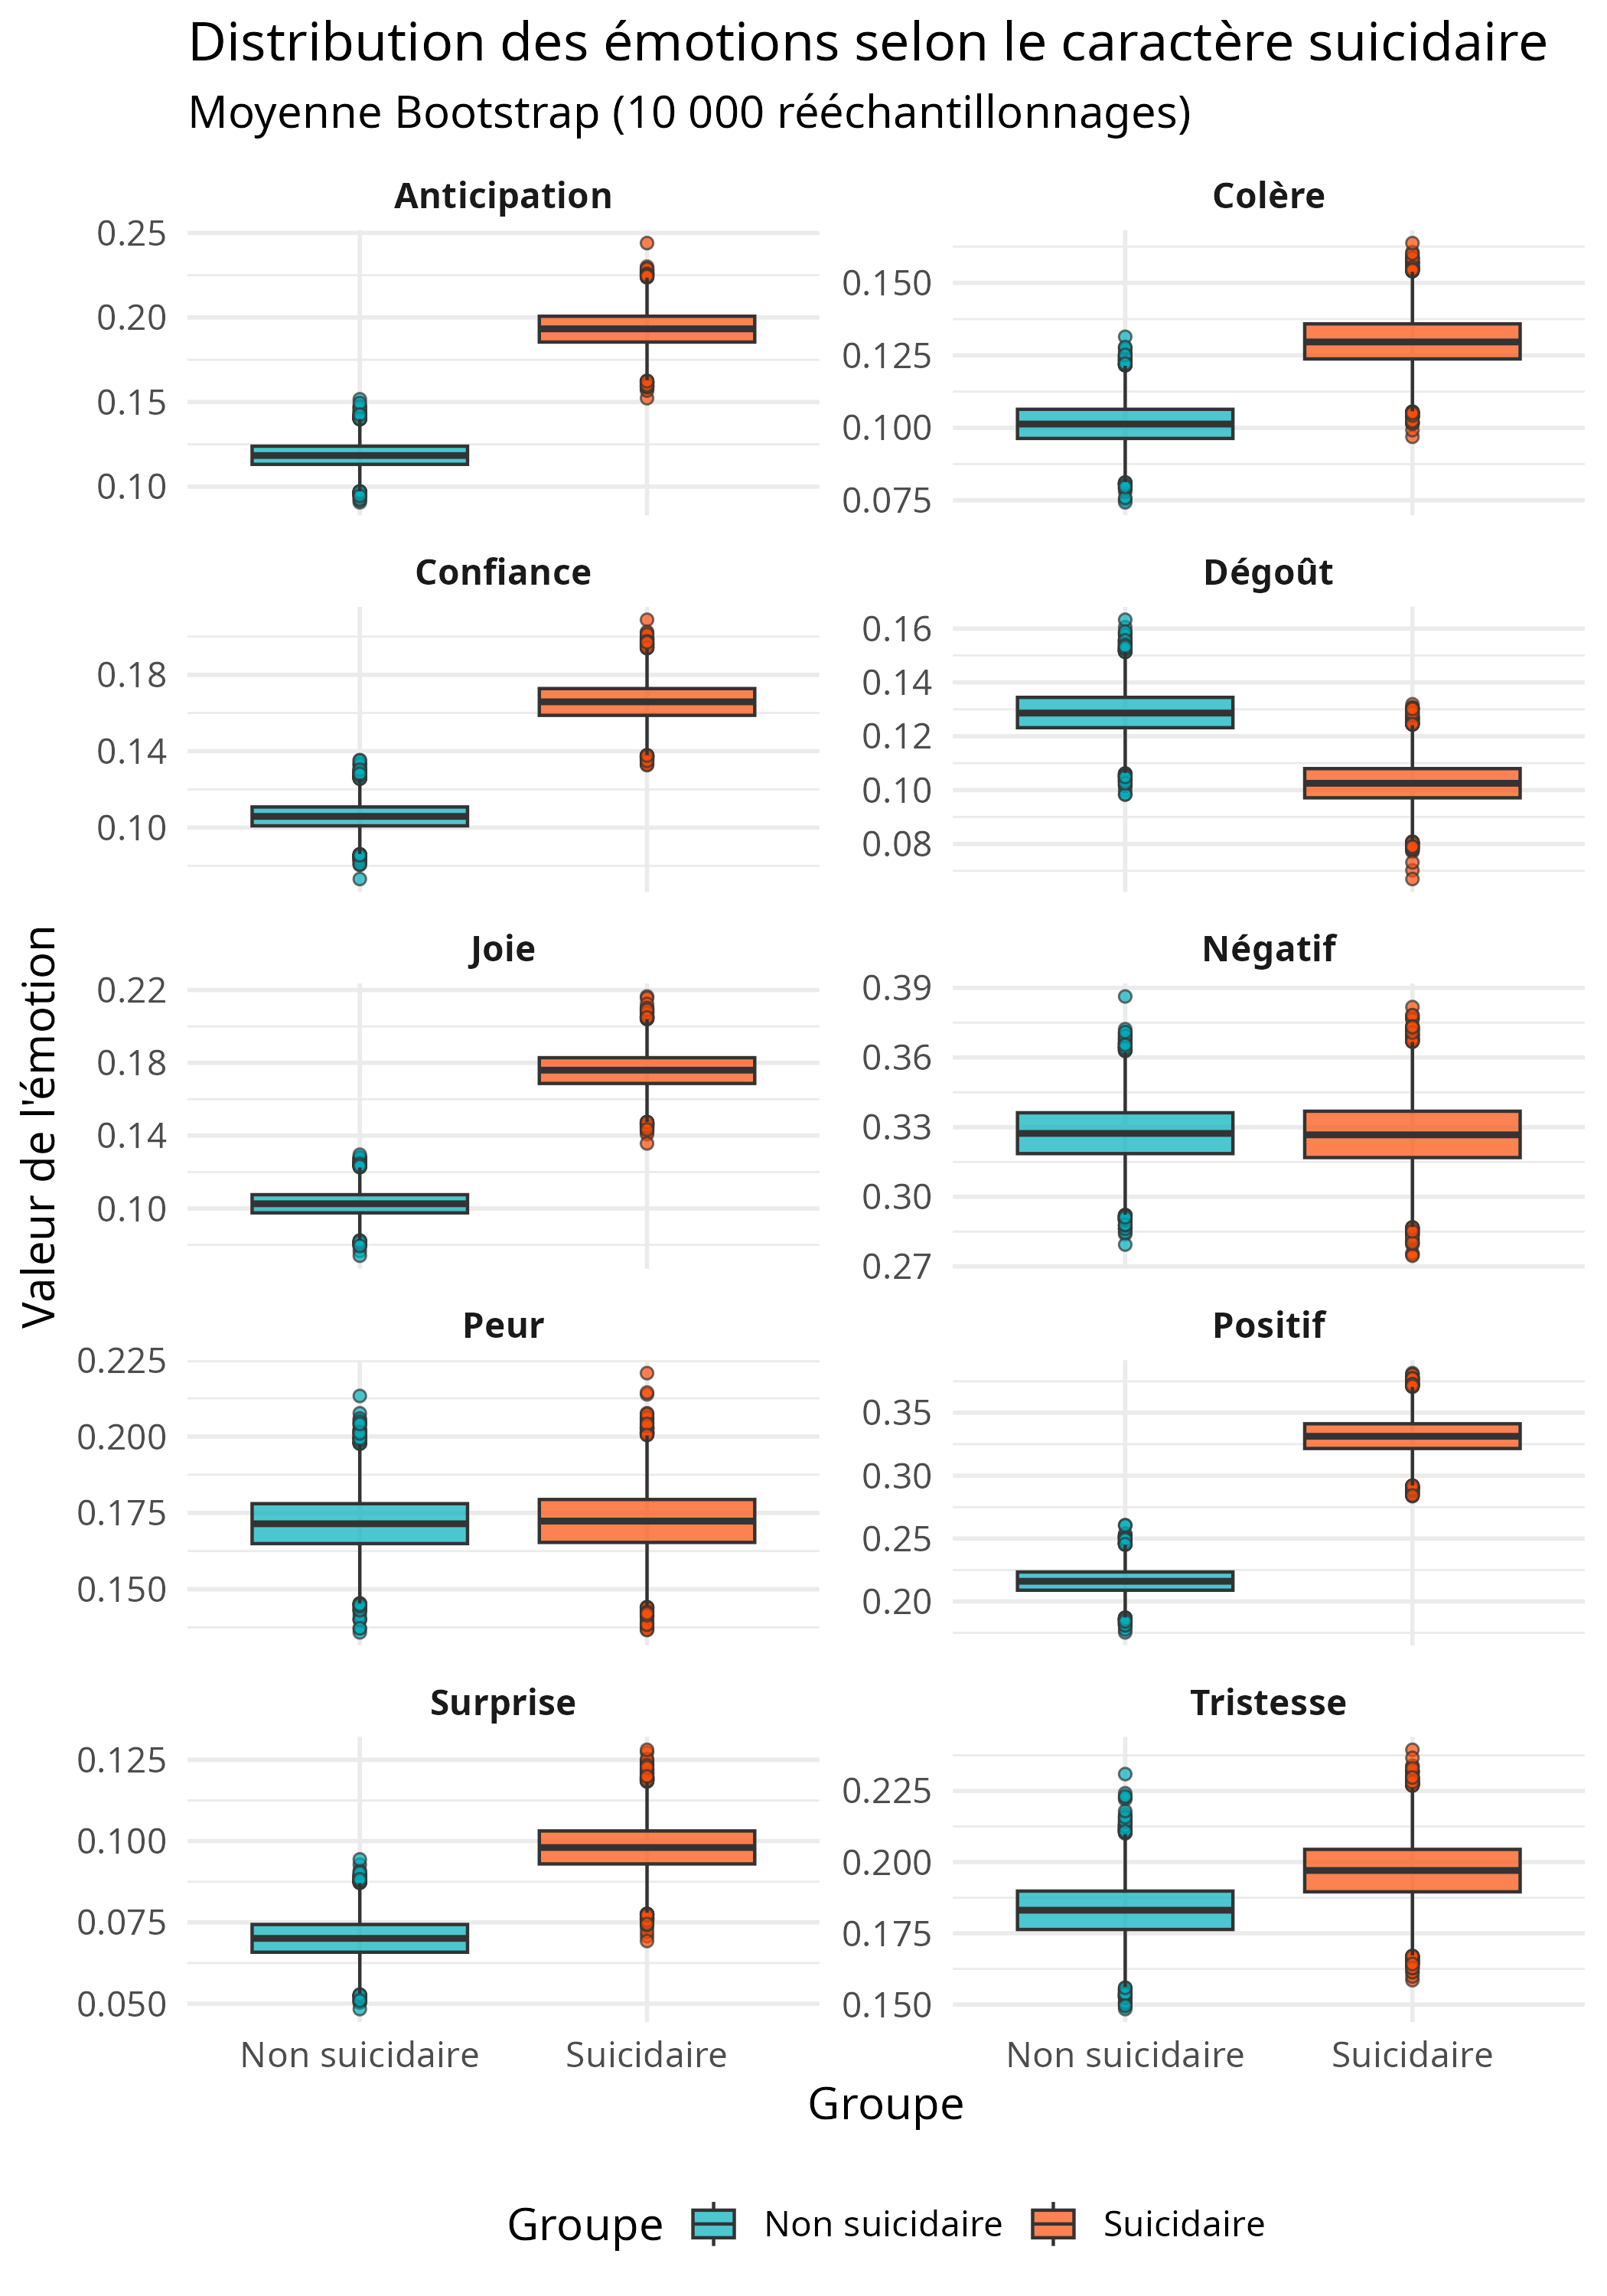
\includegraphics[width=0.8\textwidth]{images/boxplot-emotions-suicidal-bootstrap-10000.png}
	\caption{Distribution des émotions selon le caractère suicidaire (\emph{moyennes bootstrapées, 10\,000 rééchantillonnages}).}
	\label{fig:boxplot-emotions-suicidal-bootstrap}
\end{figure}

\noindent


\subsubsection{Projection des données sur les deux premiers axes (ACP)}

Pour évaluer l’éventuelle différenciation globale entre poètes suicidaires et non suicidaires, 
une analyse en composantes principales (ACP) a été réalisée sur les variables numériques
(émotions principales). La Figure~\ref{fig:pca-plot} illustre la distribution des individus 
sur le premier plan factoriel (PC1 et PC2).

\begin{figure}[H]
	\centering
	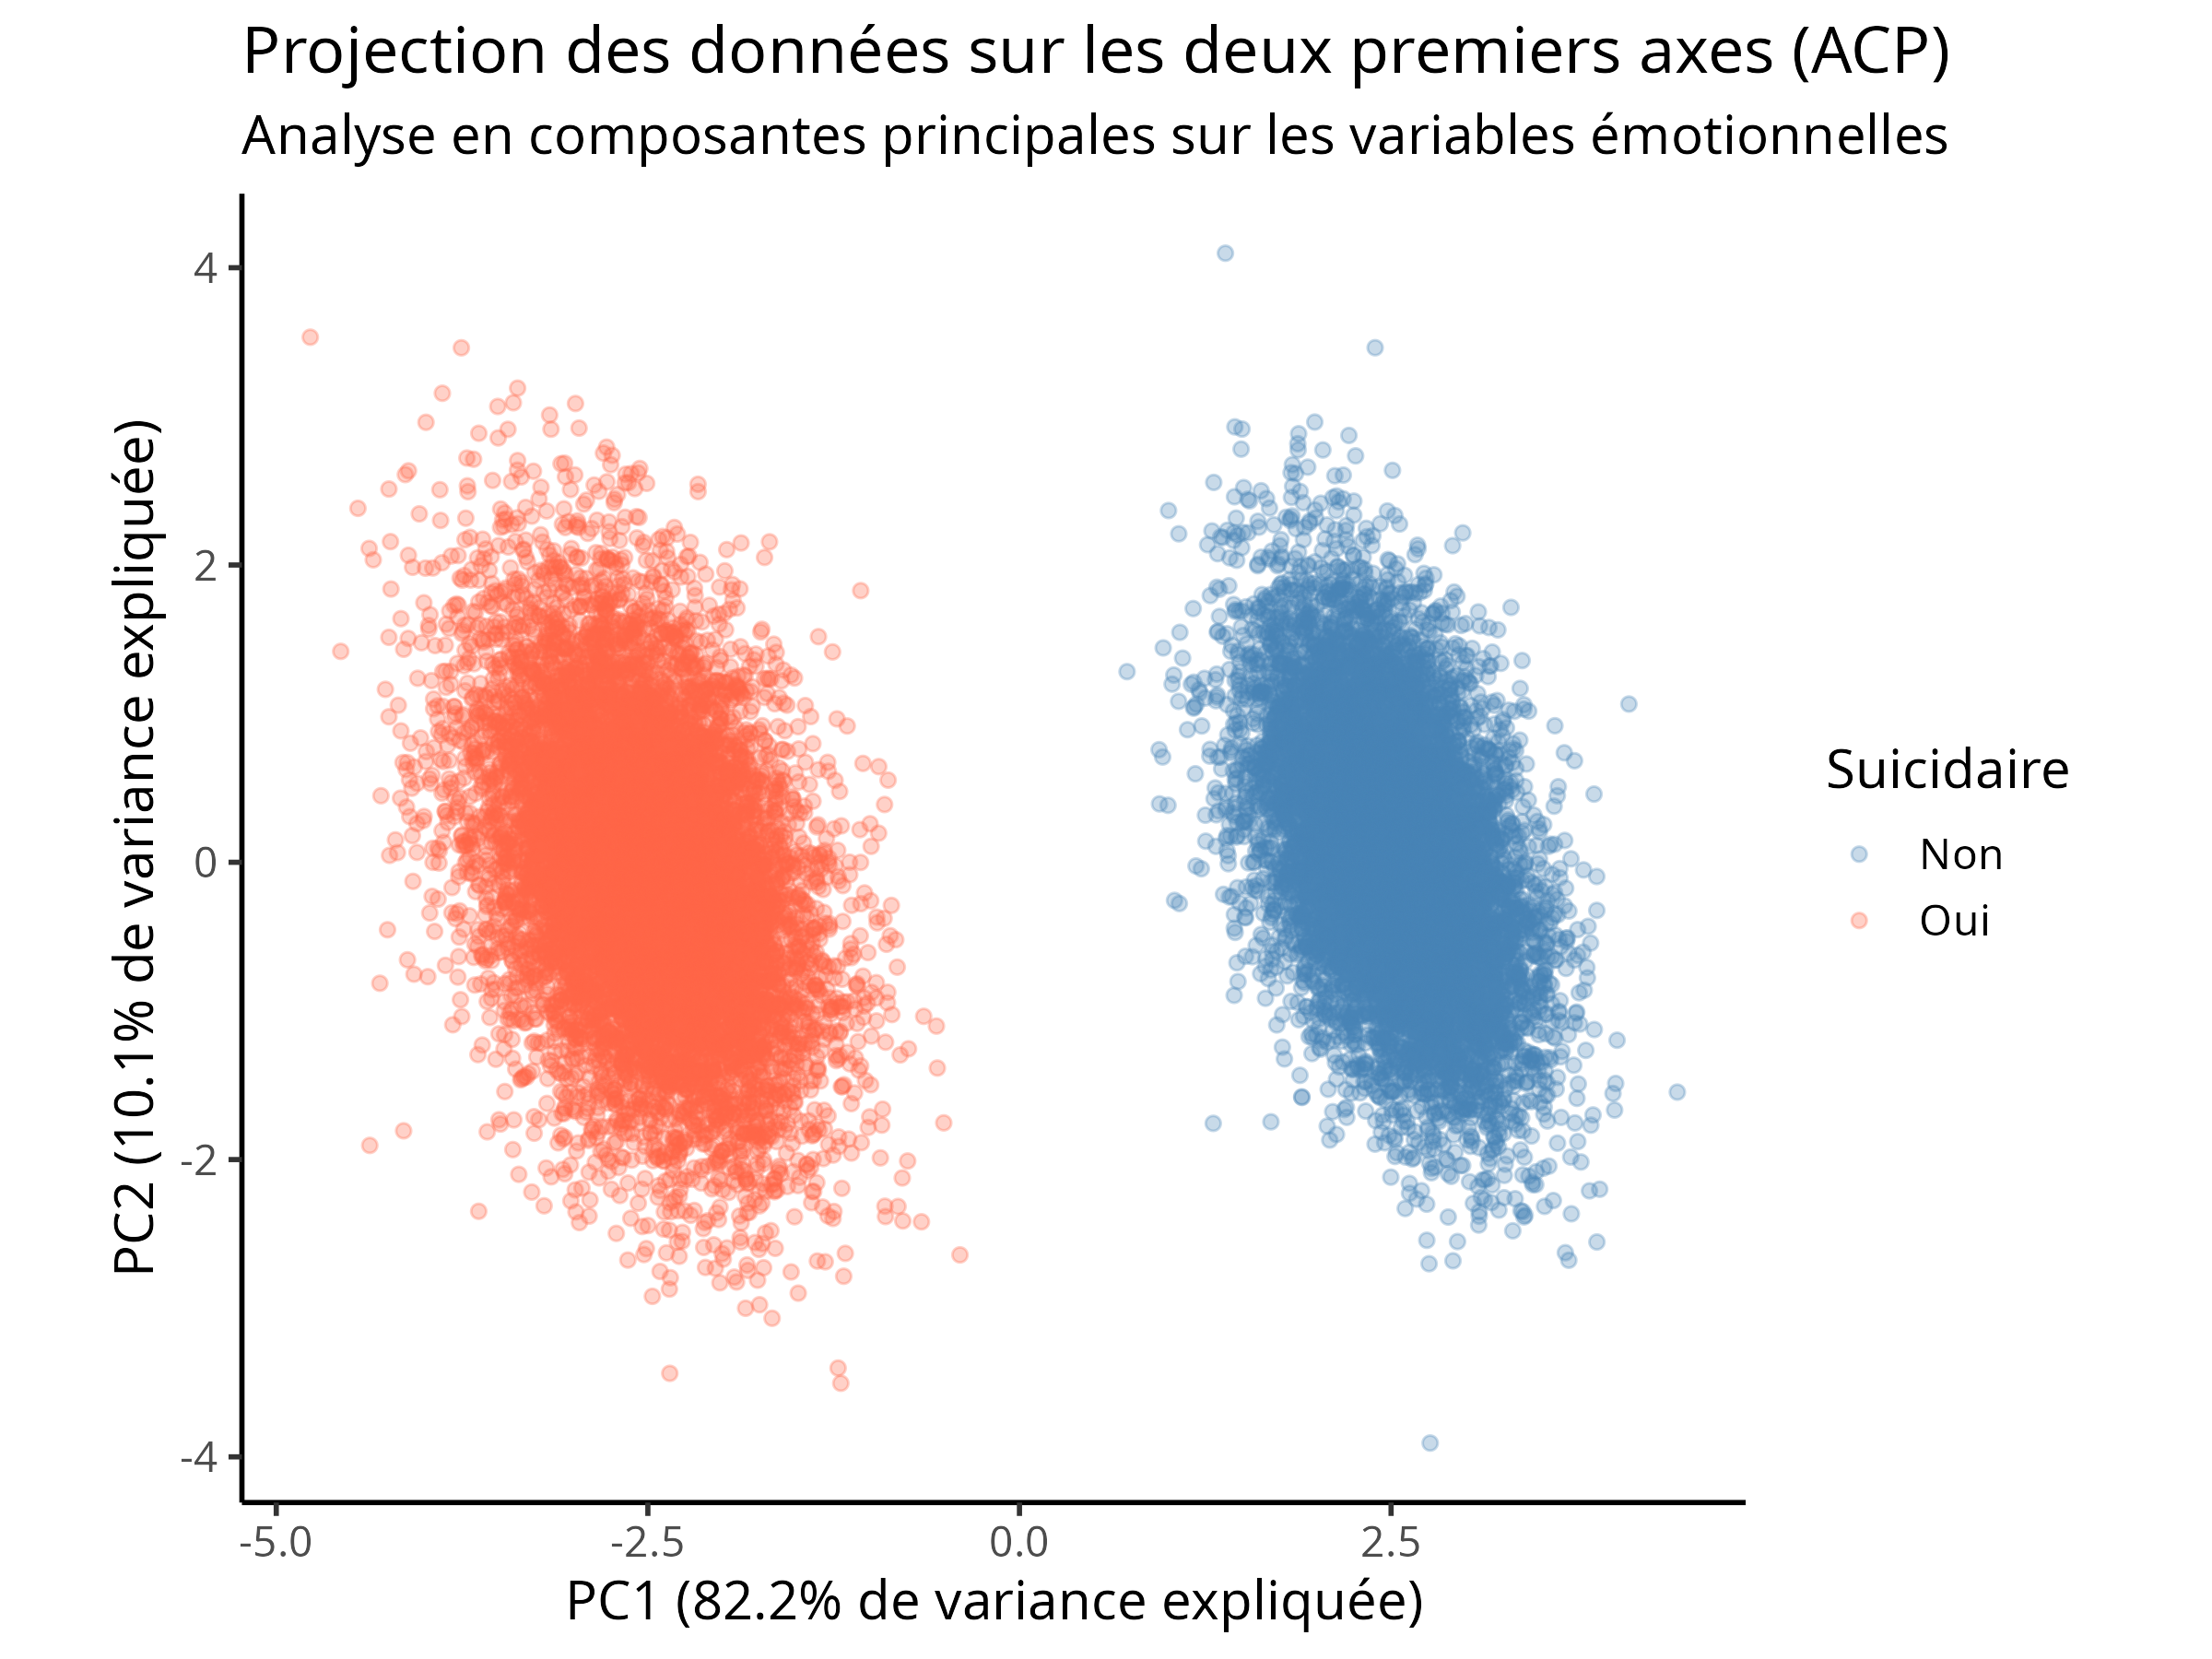
\includegraphics[width=0.8\textwidth]{images/pca_plot.png}
	\caption{Projection des données sur les deux premiers axes (ACP). 
		Les individus sont coloriés selon la variable \texttt{suicidal} 
		(\og\, Oui \fg{} pour suicidaire, \og\, Non \fg{} pour non suicidaire).}
	\label{fig:pca-plot}
\end{figure}




